\documentclass[a4paper,12pt]{article}			%Die Dokumentenklasse ist "article" mit den Einstellungen, dass das Dokument im DIN A4 Format und mit standardmäßiger Schriftgöße von 12pt erstellt wird.
\usepackage[paper=a4paper,left=35mm,right=25mm,top=25mm,bottom=20mm]{geometry}
\linespread{1.5}						%Zeilenabstand 
\usepackage[ngerman]{babel}				%Sprachpaket Deutsch
\usepackage[utf8]{inputenc}				%für die Darstellung von Umlauten
\usepackage{amsmath}					%für Matheumgebungen
\usepackage{amssymb}					%für mathematische Symbole
\usepackage{tikz}						%für Graphen (und vieles mehr)
\usepackage{enumitem}					%für Auflistungen
\usepackage{cite}						%für Zitate
\usepackage{natbib}						%für den Zitierstil
\usepackage{graphicx}
\usepackage{float}



\begin{document}
\parindent0cm 							% verhindert das Einrücken von Absätzen 

%===================================================================================
%---------------------------- Titelseite -------------------------------------------
%===================================================================================

% Hier wird die Titelseite gebastelt
% Zuerst wird die Seite auf empty eingestellt, das heißt sie hat keine Seitenzahl und auch keine Kopf- bzw. Fußzeile
\thispagestyle{empty}

\begin{center} 							%Der Text wird zentriert.

\begin{large} 
GYMNASIUM OTTOBRUNN	\\
\vspace{1cm}
Oberstufenjahrgang 2017/19\\
\vspace{1cm}
Seminarfach Softwareentwicklung\\
\vspace{2cm}
Seminararbeit\\
\end{large}

\vspace{1cm}

\begin{Huge}							%Der Text wird riesig groß!
\textbf{36. Bundeswettbewerb Informatik \\ \vspace{0.8cm}
Runde 2 \\ \vspace{0.8cm}
Aufgabe 1 und 3}\vspace{2cm}
\end{Huge}
	


\begin{large}							%Der Text wird groß.
\begin{tabular}{rl}						%Das ist eine Tabelle ohne Trennlinien. Die erste Spalte ist rechts- (r), die zweite linksbündig (l).
Verfasser:& Jonas Fritsch \\			%"&" heißt "neue Spalte", "\\" heißt "neue Zeile"
Seminarleiter: & StD Peter Brichzin \\
Bewertung:  & ......... Punkte  \\
Unterschrift des Seminarleiters: & ...........................................  \\
\end{tabular} 
\end{large}

\end{center}							%Der Text wird nicht mehr zentriert.

%===================================================================================
%---------------------------- Inhaltsverzeichnis -----------------------------------
%===================================================================================				

\newpage 								%Fängt eine neue Seite an.

\thispagestyle{empty}
\tableofcontents 						%Befehl erzeugt aus den Überschriften automatisch das Inhaltsverzeichnis!


\setcounter{page}{1}					%sagt: Zähl die Seiten erst ab hier!

%===================================================================================
%-------------------------------- Einleitung ---------------------------------------
%===================================================================================

\newpage
\section{Einleitung}



Lorem ipsum dolor sit amet, consectetur adipiscing elit. Sed tempus consectetur lorem, imperdiet dignissim est auctor a. Vivamus convallis, leo et iaculis egestas, nunc massa porttitor tellus, id faucibus urna justo eget massa. Praesent quis feugiat odio. Nullam quis mattis enim. Fusce volutpat odio in enim sodales venenatis. Mauris consequat.

%===================================================================================
%-------------------------------- Aufgabe 1 ----------------------------------------
%===================================================================================

\newpage
\section{Aufgabe 1 - "Die Kunst der Fuge"}



\subsection{Aufgabenstellung}
Ilona besitzt einen riesigen Haufen Holzklötzchen: Diese haben alle dieselbe Höhe und Tiefe,
aber verschiedene Längen. \\
Ilona möchte eine Mauer bauen. Jede Reihe der Mauer soll aus n Klötzchen bestehen, die die
Längen 1 bis n haben und lückenlos aneinander liegen. Die Stellen zwischen den Klötzchen heißen
Fugen. Ilona möchte, dass in der fertigen Mauer niemals zwei Fugen übereinander liegen,
selbst wenn sich mehrere Reihen dazwischen befinden. Außerdem soll ihre Mauer möglichst
hoch sein. \\
Für n = 4 gelingt es ihr recht schnell, eine Mauer mit drei Reihen zu bauen:
\begin{figure}[H]
    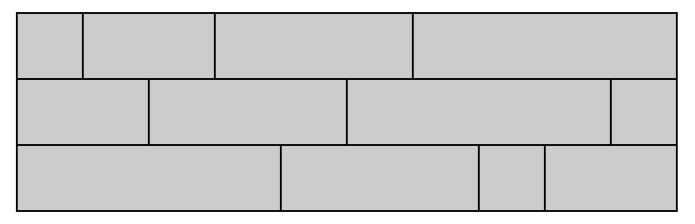
\includegraphics[width=0.7\linewidth]{Bilder/Aufgabe1/Aufgabenstellung_BeispielMauer.png}
\end{figure}
\begin{large}
    Aufgabe \\
\end{large}
Hilf Ilona, indem du ein Programm schreibst, das nach Eingabe von n eine nach ihren Vorgaben
konstruierte, möglichst hohe Mauer ausgibt. Für n = 10 sollte dein Programm eine Mauer der
Höhe 6 ausgeben können. Wie hoch werden die Mauern deines Programms für größere n?

\subsection{Lösungsidee}

\subsection{Implementierung}

\subsection{Laufzeitanalyse}

\subsection{Optimierungsmöglichkeiten}

\subsection{Beispiele}

\subsection{Quellcode}

%===================================================================================
%-------------------------------- Aufgabe 3 ----------------------------------------
%===================================================================================

\newpage
\section{Aufgabe 3 - "Quo vadis, Quax?"}



\subsection{Aufgabenstellung}

\subsection{Lösungsidee}

\subsection{Teilaufgabe (a)}

\subsection{Teilaufgabe (b)}

\subsection{Teilaufgabe (c)}
\subsubsection{Implementierung}
\subsubsection{Laufzeitanalyse}
\subsubsection{Optimierungsmöglichkeiten}
\subsubsection{Beispiele}

\subsection{Teilaufgabe (d)}

\subsection{Quellcode}

%===================================================================================
%---------------------------------- Fazit ------------------------------------------
%===================================================================================

\newpage
\section{Fazit}



Lorem ipsum dolor sit amet, consectetur adipiscing elit. Sed tempus consectetur lorem, imperdiet dignissim est auctor a. Vivamus convallis, leo et iaculis egestas, nunc massa porttitor tellus, id faucibus urna justo eget massa. Praesent quis feugiat odio. Nullam quis mattis enim. Fusce volutpat odio in enim sodales venenatis. Mauris consequat.

%===================================================================================
%--------------------------- Abbildungsverzeichnis ---------------------------------
%===================================================================================

\newpage
\section{Abbildungsverzeichnis}



Lorem ipsum dolor sit amet, consectetur adipiscing elit. Sed tempus consectetur lorem, imperdiet dignissim est auctor a. Vivamus convallis, leo et iaculis egestas, nunc massa porttitor tellus, id faucibus urna justo eget massa. Praesent quis feugiat odio. Nullam quis mattis enim. Fusce volutpat odio in enim sodales venenatis. Mauris consequat.

%===================================================================================
%--------------------------- Literaturverzeichnis ----------------------------------
%===================================================================================

\newpage
\section{Literaturverzeichnis}



Lorem ipsum dolor sit amet, consectetur adipiscing elit. Sed tempus consectetur lorem, imperdiet dignissim est auctor a. Vivamus convallis, leo et iaculis egestas, nunc massa porttitor tellus, id faucibus urna justo eget massa. Praesent quis feugiat odio. Nullam quis mattis enim. Fusce volutpat odio in enim sodales venenatis. Mauris consequat.

%===================================================================================
%------------------------- Erklärung des Verfassers --------------------------------
%===================================================================================

\newpage
\section{Erklärung des Verfassers}



Lorem ipsum dolor sit amet, consectetur adipiscing elit. Sed tempus consectetur lorem, imperdiet dignissim est auctor a. Vivamus convallis, leo et iaculis egestas, nunc massa porttitor tellus, id faucibus urna justo eget massa. Praesent quis feugiat odio. Nullam quis mattis enim. Fusce volutpat odio in enim sodales venenatis. Mauris consequat.



\end{document}